\documentclass{article}
\usepackage{microtype,graphicx,booktabs,hyperref,amsmath}
\newcommand{\theHalgorithm}{\arabic{algorithm}}
\usepackage[preprint]{icml2026}
\icmltitlerunning{Calibration Admission Requires Mechanical Qualification}
\makeatletter\gdef\icmlcorrespondingauthor@text{Author details pending}\makeatother
\begin{document}\twocolumn[
\icmltitle{Calibration Admission Requires Mechanical Qualification:\\Four Complete Native Simulation Trials with Retained Failures}
\begin{icmlauthorlist}\icmlauthor{Research development draft}{draft}\end{icmlauthorlist}
\icmlaffiliation{draft}{Negative-result component supplement; no full learning-system claim}\vskip .3in]
\printAffiliationsAndNotice{}
\begin{abstract}
Physical-time scheduling is meaningful only when the preserved skill can
produce the required effective events. Four frozen Isaac Sim/PhysX FR3 calibration
trials complete all commands and pass independent raw consistency checks.
Two lighter-payload trials complete manipulation; two heavier-payload trials
lose transport grasp and have no stable-release endpoint. All four remain
in the calibration denominator. Consequently no interval fit or held-out
timing test is admitted. These retained negative observations expose a
mechanical qualification gap rather than a demonstrated scheduling or
learning improvement.
\end{abstract}

\section{Protocol and complete result}
The preserved Isaac Sim 5.1/PhysX A-r7 scene contains 56 rigid bodies and nine articulations.
The FR3 executes the original bottle skill with physical mass/inertia factors
0.8 or 1.2 and a position-target FIFO of zero or 12 ticks at 240 Hz.
Gravity compensation and state guards remain immediate. A prospective
118-file execution release, four-case calibration roster and original
mechanical thresholds are fixed before trials. Every case is a fresh,
uninterrupted native epoch; no task-period object or joint state write occurs.

\begin{table}[h]\centering\small
\caption{All four calibration cases, with missing endpoints retained.}
\begin{tabular}{rrrrl}\toprule
Mass & FIFO & Samples & Mechanic & Release\\\midrule
0.8 & 0 & 13,427 & TRUE & Observed \\
0.8 & 12 & 13,439 & TRUE & Observed \\
1.2 & 0 & 13,427 & FALSE & Missing \\
1.2 & 12 & 13,439 & FALSE & Missing \\
\bottomrule\end{tabular}\end{table}
The trials contain 53,732 task samples and 36 actual RGB snapshots. Resource
allocation is bounded by 0.40953 GPU hours, including worker startup.
All contact response intervals are approximately 171--175 ms. Light-case
stable-release responses are 88--92 ms; heavy-case endpoints are absent.
Calibration uses the original unscheduled skill, whose timing is early;
command completion is not timing success. Four attempted calibration cases
cannot be replaced by the two mechanically eligible cases. The interval
fit is absent, and zero of the planned 16 timing tests has run.

\section{Independent failure localization}
Raw clocks, queues, controls, contacts, states, events and existing scores
are independently recomputed. Both heavy cases acquire and lift the bottle,
then lose relative-pose/contact continuity and tilt acceptance during
transport. Only the zero-FIFO heavy case later collides with another bottle;
collision is not the common failure cause. The paired robot TCP discrepancy
is below 0.04 mm, while the bottle drift is large. This localizes grasp loss
but does not establish a causal actuator or friction diagnosis.

For light cases, 13 strict-hold negative samples occur between commanded
opening and composite stable-release onset, with none before opening.
The unchanged diagnostic therefore cannot be interpreted as premature
grasp loss. Main mechanics, event gaps and strict hold retain their
prospective separate definitions.

\begin{figure*}[t]\centering
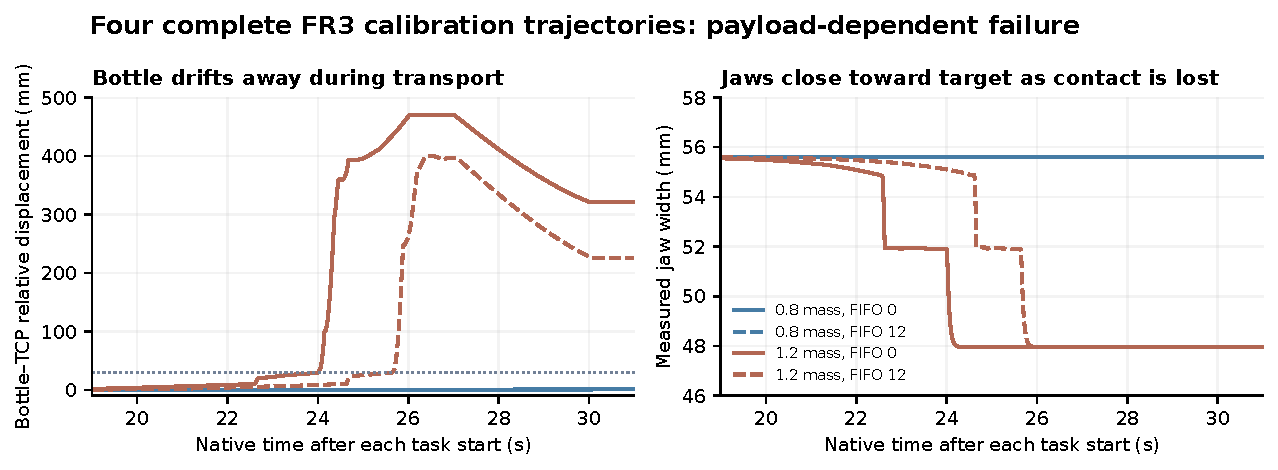
\includegraphics[width=.82\textwidth]{payload_failure.pdf}
\caption{Actual native state observations from all four trials. Local task
time aligns separate epochs; no cross-epoch continuity is asserted.}
\end{figure*}

An initial auditor incorrectly demanded bitwise equality between requested
and installed inertia. Its rejection is retained. The new auditor applies
the originally frozen installation tolerance ($10^{-6}$ relative,
$10^{-10}$ absolute for inertia); all state, queue, score and event checks
remain exact. This audit-contract repair does not remove the two physical
transport failures.

\section{Core precedents and next hypothesis}
MATTERIX already provides waiting, temporal process semantics, concurrent
agents, workflow verification and HSM skills \cite{matterix}. Its heating
example distinguishes power-off from subsequent reaction completion.
Auto-Engineering likewise provides engineering harnesses, BC/DAgger and
deployment-artifact reuse. These are precedents rather than our new
principles. A full paper must demonstrate independently calibrated tight
contracts, valid recovery under an original external event, and shared
actor absorption against strong HSM/scheduling and matched relabeling.
The earlier twin-rotor counterfactual-reference component is not that
external-event recovery test.

A separate candidate qualification is proposed: preserve the original
scene/drive restoration, install and measure one hand-stiffness change
before the task, and keep mass, targets, friction and mechanical criteria
fixed. A subsequent separate one-case qualification passes these mechanics
but lacks before-change damping/effort arrays and state-token preimages.
It does not prove a causal root cause or provide a complete independent
three-snapshot installation audit. A new source with complete logging must
pass all four fresh calibration cases before timing tests.
New success never rewrites the retained old failures. No new policy
weights, chemical endpoints or real robot trials are credited here.

\begin{thebibliography}{9}
\bibitem[Darvish et~al.(2026)]{matterix} Darvish, K., et al. MATTERIX: toward a digital twin for robotics-assisted chemistry laboratory automation. \emph{Nature Computational Science}, 6:67--82, 2026. \url{https://doi.org/10.1038/s43588-025-00924-4}.
\end{thebibliography}
\end{document}
